% Map of the West Indies
\begin{figure}[H]
    \centering
	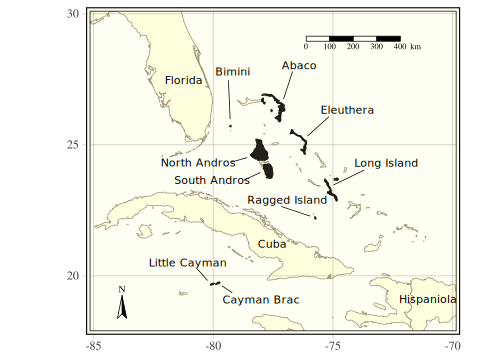
\includegraphics[width=0.8\textwidth]{../maps/map.pdf}
	\caption{Map of the West Indies with sampled islands highlighted in black.}
	\label{fig:map}
\end{figure}

% Boxplots and analyses of variance
\begin{sidewaysfigure}
	\centering
	\includegraphics[width=18cm]{../analyses/07-ANOVA/figure_anova.png}
	\caption{Dewlap color variation between habitat-types across the most significant islands. (A) Mapping of reflectance at various wavelengths onto the principal components (loadings from the PCA rotation matrix). (B) Distribution of PC scores between habitats along the first four PCs on each island where significant between-habitat differences were detected using SVMs. P-values are reported for univariate ANOVA (or Kruskal-Wallis tests when applicable, see Methods). Post hoc significant differences at a 0.05 error rate are indicated with horizontal bars. *, P < 0.05.}
	\label{fig:anova}
\end{sidewaysfigure}

% Classification accuracy of SVMs
\begin{figure}[H]
    \centering
	\includegraphics[width=\textwidth]{"../analyses/04-machine learning/plots/classif_svm_pca"}
	\caption{SVM classification accuracy across islands based on principal component data. Histograms show accuracy distributions over 100 replicates for each five cross-validation bins per island. The dashed line is the density of a corresponding null binomial distribution, which would be expected under random guessing (testing sets with 20\% of the observations for each island and success probability of $1/3$). Inset plots show the corresponding average confusion matrices and represent the proportion of lizards from each habitat (columns) reassigned in each other habitat (rows), with an interpretation guide in the right panel. Binomial test P-values indicate deviations of the mean classification accuracy to the null distribution. *, P < 0.05.}
	\label{fig:classif-svm-pca}
\end{figure}
